\documentclass[12pt]{article}
\usepackage[margin=1in]{geometry}
\usepackage[utf8]{inputenc}
\usepackage{amsfonts}
\usepackage{amsmath}
\usepackage{amsthm}
\usepackage{tikz-cd}
\usepackage{tipa}
\usepackage{graphicx}
\usepackage{float}

%%% Common categories
\newcommand{\tp}{\;\mathrm{type}}
\newcommand{\Hom}{\mathrm{Hom}}
\newcommand{\G}{\Gamma}
\newcommand{\pit}[1]{\prod_{(#1)}} % pi-type
\newcommand{\pitxa}{\pit{x:A}}
\newcommand{\sit}[1]{\sum_{(#1)}} % sigma-type
\newcommand{\ent}{\vdash}
\newcommand{\adj}{\dashv}
\newcommand{\refl}{\ensuremath{\textsf{refl}}}
\newcommand{\ap}{\ensuremath{\textsf{ap}}}
\newcommand{\ind}{\ensuremath{\textsf{ind}}}
\newcommand{\lift}{\ensuremath{\textsf{lift}}}
\newcommand{\inv}{\ensuremath{\textsf{inv}}}
\newcommand{\concat}{\ensuremath{\textsf{concat}}}
\newcommand{\transport}{\ensuremath{\textsf{transport}}}
\renewcommand{\sec}{\ensuremath{\textsf{sec}}}
\newcommand{\retr}{\ensuremath{\textsf{retr}}}
\newcommand{\total}{\ensuremath{\textsf{total}}}
\newcommand{\isequiv}{\ensuremath{\textsf{is\_equiv}}}
\newcommand{\fib}{\ensuremath{\textsf{fib}}}
\newcommand{\id}{\ensuremath{\text{id}}}
\newcommand{\judgeq}{\ensuremath{:\equiv}}
\newcommand{\reflfx}{\ensuremath{\refl_{f(x)}}}

\newcommand{\rr}{\ensuremath{\mathbb{R}}}
\newcommand{\rrn}{\ensuremath{\mathbb{R}^n}}
\newcommand{\rrm}{\ensuremath{\mathbb{R}^m}}
\newcommand{\rrx}{\ensuremath{\mathbb{R}[x]/x^2}}
\newcommand{\rry}{\ensuremath{\mathbb{R}[y]/y^2}}
\newcommand{\cc}{\ensuremath{\mathbb{C}}}
\newcommand{\nn}{\ensuremath{\mathbb{N}}}
\newcommand{\dd}{\ensuremath{\mathbb{D}}}
\newcommand{\vv}{\ensuremath{\mathbb{V}}}
\newcommand{\cinfty}{\ensuremath{C^{\infty}}}
\newcommand{\smfd}{\textsf{SmoothMfd}}
\newcommand{\calg}{\textsf{CAlg}_{\rr}}
\newcommand{\cart}{\textsf{CartSp}}
\newcommand{\formalcart}{\textsf{FormalCartSp}}
\newcommand{\formalsmoothset}{\textsf{FormalSmoothSet}}
\newcommand{\smoothset}{\textsf{SmoothSet}}
\newcommand{\setcat}{\textsf{Set}}
\newcommand{\psh}[1]{\textsf{Psh}(#1)}
\newcommand{\sh}[1]{\textsf{Sh}(#1)}
\newcommand{\pshcart}{\psh{\cart}}
\newcommand{\rmodal}{\Re}
\newcommand{\imodal}{\Im}
\newcommand{\shape}{\ensuremath{\text{\textesh}}}
\newcommand{\op}[1]{#1^{\textsf{op}}}
\newcommand{\pt}{\mathrm{pt}}
\newcommand{\Aut}{\mathrm{Aut}}
\newcommand{\BAut}{\mathrm{BAut}}
\newcommand{\im}{\mathrm{im}}
\newcommand{\Fin}{\mathrm{Fin}}
\newcommand{\Type}{\mathrm{Type}}

\newcommand{\bg}{\ensuremath{\textbf{B}G}}
\newcommand{\bgconn}{\ensuremath{\textbf{B}G_{\textsf{conn}}}}
\newcommand{\bgdiff}{\ensuremath{\textbf{B}G_{\textsf{diff}}}}

\newcommand{\gc}[1]{\marginpar{\bf $\leftarrow$ {#1}}}
%\newcommand{\gc}[1]{}

\newtheorem{mydef}{Definition}
\newtheorem{mythm}{Theorem}
\newtheorem{mylemma}{Lemma}
\newtheorem{myprop}{Proposition}
\newtheorem{myclaim}{Claim}

\title{Categories and modalities for smoothness}
\author{Greg Langmead}
\begin{document}
\maketitle
\begin{abstract}
Differential cohesion and modal HoTT promise to give access to constructions from differential geometry. In this series of talks I will tell a story that takes us from the classical definition of a smooth manifold to differential cohesion in a category where we can interpret modal HoTT. I will assume only basic topology and category theory and will provide details that are sometimes waved away. I will also motivate the study of smooth manifolds as a worthy field with surprising results and tough open questions such as the smooth four-dimensional Poincaré conjecture.
\end{abstract}
\tableofcontents
\section{Introduction}\label{sec:introduction}
As someone ``classically trained'' in differential geometry, my recent adventures in homotopy type theory have made me very excited to explore an entirely new angle on a topic I love. It is the case today that modal HoTT allows us to access smoothness and prove theorems about manifolds, Lie groups and more. In order to participate in this new and exciting field, someone like me needs a bridge. More than one, in fact. The current document is intended as one of those bridges. Starting from the classical definition of a smooth manifold and the category containing these objects and the smooth maps between them, we will define several enlargements of the category until we arrive at something where modal HoTT can be interpreted.

To make the most of this process, we will always try to keep track of where smoothness is entering in. It's not always obvious!

\begin{mydef}\label{def:smoothmfd}
A smooth manifold is a Hausdorff topological space $M$ with countable basis, and with a maximal smooth atlas. An atlas is a covering of $M$ by open sets $U_i$, each of which is the image of a homeomorphism $f_i:\mathbb{R}^n\to M$ (called a \emph{chart}), such that $f_j^{-1}\circ f_i$ is smooth wherever it is defined. Two atlases are compatible if their union is again an atlas. The maximal atlas is the union of all compatible atlases.
\end{mydef}

Note that this definition expresses $M$ as a colimit of a diagram of arrows from $\rr^n\to M$, more specifically a pushout. More on this shortly.

A continuous function $f:M\to N$ between two smooth manifolds is defined to be smooth if the appropriate composition with charts is a smooth function between cartesian spaces.

The category \smfd\ has objects the smooth manifolds of any finite dimension, and morphisms the smooth maps.

This category, innocuous though it seems, has some strange properties! There are topological manifolds that are missing from it, and some that are way over-represented! You can't just take a topological manifold and assume you can give it a unique maximal smooth atlas and stick it into \smfd.

The table below contains some examples.

\begin{center}
\label{table:smoothstructures}
\begin{tabular}{|l|l|}
\hline
kind of manifold & number of inequivalent smooth atlases \\ \hline
dim $\leq 3$ & 1 \\ \hline
dim $\geq 5$ & $\geq 0$, finite \\ \hline
$\rr^n, n\neq 4$ & 1 \\ \hline
$\rr^4$ & uncountably many \\ \hline
$S^4$ & unknown, $\geq 1$ \\ \hline
dim $= 4$, compact without boundary & $\geq 0$, at most countably many \\ \hline
dim $= 4$, otherwise & $\geq 1$, at most uncountably many \\ \hline
\end{tabular}
\end{center}

The claim that $S^4$ has exactly one smooth structure is known as the four-dimensional smooth Poincaré conjecture. Its status is ``extremely unknown''. For more of the beautiful story around four-dimensional topology and smooth structures see the accessible and detailed book by Scorpan \cite{scorpan_wild_2005}.

The spheres behave surprisingly as well.

\begin{center}
\label{table:smoothspheres}
\begin{tabular}{|l|p{4cm}|}
\hline
$n$ & number of inequivalent smooth atlases on $S^n$ \\ \hline
1 & 1 \\ \hline
2 & 1 \\ \hline
3 & 1 \\ \hline
4 & $\geq 1$ \\ \hline
5 & 1 \\ \hline
6 & 1 \\ \hline
7 & 28 \\ \hline
8 & 2 \\ \hline
9 & 8 \\ \hline
10 & 6  \\ \hline
11 & 992  \\ \hline
12 & 1 \\ \hline
13 & 3 \\ \hline
14 & 2 \\ \hline
15 & 16256 \\ \hline
16 & 2 \\ \hline
17 & 16 \\ \hline
18 & 16 \\ \hline
19 & 523264 \\ \hline
20 & 24 \\ \hline
\end{tabular}

(from https://en.wikipedia.org/wiki/Differential\_structure)
\end{center}

Is \smfd\ a nice category? It does have finite products (cartesian product) and coproducts (disjoint unions). Manifolds are themselves certain colimits. However in this category does not have all limits or colimits, nor is it cartesian closed.

For example, consider the equalizer $\left\{(x, y) | xy = 0\right\}\subset \rr^2$. As a set this must be equal to the union of the $x$-axis and $y$-axis. But this cannot be given the structure of a topological manifold nor a smooth one, due to the failure to be homeomorphic to any $\rr^n$ at the origin. Full argument: the forgetful functor $U:\smfd\to\setcat$ preserves limits and colimits as it has both left and right adjoints. The equalizer as a set is this union of axes, and so the manifold must have that underlying set. But this set cannot be promoted to a smooth manifold.

Consider the coequalizer $\left(\mathbb{R}^2 \coprod \mathbb{R}\right)/(0,0)\sim 0$. Similarly this cannot be given the structure of a topological manifold nor a smooth one, also at the origin.

Is \smfd\ cartesian closed, i.e. does it contain function spaces of smooth maps? This has been attempted with some success, but we'll skip over that story because we're going to do it with sheaves later. In fact right now.

\section{Sheaves on \cart}\label{sec:sheaves}

My take on presheaves and sheaves is inspired by Daniel Dugger's informal notes \emph{Sheaves and Homotopy Theory}\cite{dugger_sheaves_1999}. His analogy to generators and relations is the one that clicked for me in this context.

Define \cart\ to be the full subcategory of \smfd\ containing just the $\rr^n$ for finite $n$ (recall that ``full'' means include every morphism). In the case of $\rr^4$ let's just bring the standard smooth structure. We can try to build the fake $\rr^4$s later on with surgery and such.

Due to the existence of real-valued functions such as $\frac{1}{1+e^{-x}}$ we can map all of \rr\ to the open interval $(0,1)$. So note that this category is not as pitifully empty as I, at least, thought at first. You can cover $\rr^n$ with balls each of which is a diffeomorphic image of $\rr^n$. We'll be doing just that.

To generalize \smfd\ we'll use \cart\ in a new way. In the original atlas-based definition of a smooth manifold we were characterizing manifolds by the slogan ``locally isomorphic to $\rr^n$.'' This is a way to cash out the more general concept ``modeled on $\rr^n$.'' But we will now shift to the paradigm ``can be probed by $\rr^n$'' or equivalently ``has specified maps from the test spaces $\rr^n$.'' In this framework we will specify probes from all dimensions of cartesian spaces, not just the one that has the same dimension as the manifold (if any such concept as dimension survives our shenanigans).

A \emph{presheaf} on \cart\ is a functor $$\cart^{\mathrm{op}}\to \mathrm{Set}$$ Think of one presheaf $M$ (suggestive name) as a would-be space together with the specification of what probing functions are smooth. Sometimes these probes are called \emph{plots}. These are different from charts. Charts are specific homeomorphisms that cover $M$. Here we must provide the entire set of all possible smooth functions into $M$ from $\rr^n$, for all $n$.

The category \pshcart\ consists of all such functors, together with the natural transformations between them. This is an interesting category! If $C$ is any locally small category, there is an embedding (a full and faithful functor that is injective on objects) $C\to\psh{C}$ called the \emph{Yoneda embedding}. In fact \psh{C} is the \emph{free cocompletion} of $C$, meaning it freely adds all colimits from $C$. In fact \psh{C} is a \emph{topos} which is a checklist of wonderful properties, and we'll be using them all by the end because HoTT and toposes are closely related. In a nutshell, \psh{C} inherits these nice properties from $\mathsf{Set}$.

BUT.

If $C$ already has some colimits, \psh{C} will not respect these. It is \emph{too free}.

Consider two subobjects of $\rr^n$ in \cart, say two disjoint open balls $U$ and $V$. \gc{complete the example}

Following Duggers we think of sheaves as the subcategory of presheaves that preserve the existing colimits that we had. There is an analogy to specifying a group as the quotient of a free group by a subgroup generated by some relations.

It's illustrative to understand the layers of exoticness that are introduced by moving from \smfd\ to sheaves. Manifolds embed in diffeological spaces which are the concrete sheaves (see Baez and Hoffnung \cite{baez_convenient_2008}).\gc{give these subcategories}

\section{The algebra of functions}\label{sec:algebras}

For a smooth manifold $M$ the set of smooth real-valued maps $f:M\to\rr$ has the structure of a vector space, a ring, and in fact a commutative algebra. An algebra is a vector space over a base field (hence it has a commutative addition operation) which also has a multiplication operation that satisfies the distributive law when it interacts with addition. If the multiplication is commutative then we say the algebra is commutative. In this case the operations are all pointwise and so the algebra properties are inherited from \rr. For example $fg(x)=f(x)g(x)$ where the right hand side is multiplication in \rr.

\begin{myprop}\label{prop:algebrafunctor} Taking the algebra $\cinfty(M)$ of smooth functions of a smooth manifold $M$ gives a contravariant functor $\smfd\xrightarrow[]{\cinfty}\calg^{\mathrm{op}}$.
\end{myprop}

There are important subcategories of $\calg$ that themselves contain the image of this functor, notably the ``smooth algebras'' but we won't make use of their special properties, so we might as well use the simpler larger category.

Crucially this functor is actually \emph{faithful}, meaning if you fix two manifolds then the functor is injective on the hom set between them. Said another way, any algebra homomorphism $\cinfty(N)\to\cinfty(M)$ comes from a unique smooth map $M\to N$. Therefore we can embed \smfd\ into $\calg$ and treat its image as an equivalent copy of \smfd\ (with arrows reversed) and find new ways to extend it and build new categories!

The proof of faithfulness is interesting and we will explore it fully because it's challenging to piece it together from the references that exist easily to hand today. Since we have a couple other such ``smooth facts'' to make use of let's handle them together.

\section{The lemmas about smoothness}\label{sec:smoothnesslemmas}

\begin{mylemma}\label{lemma:smoothfact1}(``Milnor's Exercise'') The map $M\xrightarrow[]{\mathrm{ev}}\Hom(\cinfty(M),\rr)=\Hom(\cinfty(M),\cinfty(\rr^0))$ given by evaluation at a point of $M$ is a bijection.
\end{mylemma}
\begin{proof}
See also Kolář, Michor and Slovák \cite{kolar_natural_1993}, especially the preamble before section 35 and Corollary 35.9. Let $\phi\in\Hom(\cinfty(M), \rr)$. Then $\ker(\phi)$ is an ideal of codimension 1. (An ideal of an algebra is a vector subspace which is closed under multiplication by an arbitrary element of the algebra.) Consider the collection of zero sets $Z_f, f\in \ker(\phi)$. This collection of sets is closed under intersection: given $Z_f, Z_g$ then $Z_{(f^2+g^2)} = Z_f\cup Z_g$ and $f^2+g^2\in\ker(\phi)$. We have satisfied some of the hypotheses of the following topological lemma:

\begin{mylemma}If $X$ is Hausdorff and $C\subseteq X$ compact, and $F=\{C_i\}$ any collection of closed subsets of $C$ with the property that $C_i, C_j\in F\implies C_i\cap C_j\in F$, then $\bigcap_i C_i \neq\emptyset$.\end{mylemma}

We have a collection of sets closed under intersection, so to satisfy the hypotheses of this new lemma it suffices to show that there is some $Z_f$ compact and nonempty, for then we can use this as the set $C$.

Suppose for a moment that we had this $Z_f$. Let's see how we can finish proving Milnor's exercise. Suppose $\bigcap_{f\in\ker(\phi)}Z_f\neq\emptyset$, and so it contains some point $x$. Now consider an arbitrary $g\in\cinfty(M,\rr)$. Construct the function $g'=g-\phi(g)1$ where the latter term means the constant function with value $\phi(g)$. Then $g'\in\ker(\phi)$, so $g'(x)=0$, i.e. $g(x)-\phi(g)1(x)=0$ and hence $\phi(g)=g(x)$, and so $\phi=\mathrm{ev}_x$ as desired.

Now to construct the function $f$ whose zero set is compact and nonempty. Back in Definition~\ref{def:smoothmfd} we assumed all our smooth manifolds are Hausdorff with countable basis. This in turn implies paracompactness, a property that was put on this Earth to supply the existence of a \emph{partition of unity}, a countable collection of smooth bump functions, each with compact support, and with the collective property that in a neighborhood of any point only finitely many of them are nonzero, and they sum everywhere to the constant function 1. So let's fix a partition of unity $\{f_i\}_{i\in\nn}$. Consider the function $$g=f_1+2f_2+3f_1+\cdots.$$
This function is everywhere positive. We claim that for every $c>0$ that $U=g^{-1}([0,c])$ is compact. By continuity $U$ is closed. And it must lie in the union of finitely many supports, as the terms $nf_n$ grow beyond $c$ eventually. So $U$ is closed and contained in a finite union of compact sets, which is compact, and so $U$ is compact. One more trick: this argument works for $g^2$ as well, possibly with a different value of $c$. Since the codimention of $\ker(\phi)$ is 1, some linear combination $f=ag+bg^2=0, a, b\in\rr$. This $f$ carves out a compact nonempty zero set. \gc{what was the gap here at the end? That a, b might be negative? Surely one of them *is* negative?}
\end{proof}
It is perhaps notable that there is a larger class of topological manifolds for which Milnor's exercise holds, which goes by the name \emph{realcompact}, in case you want to look that up.

\begin{mylemma}\label{lemma:smoothfact2} For two smooth manifolds $M_1$ and $M_2$ the map
\begin{align}
\cinfty(M_1, M_2) &\to \Hom(\cinfty(M_2),\cinfty(M_1)) \\
f &\mapsto (g\mapsto g\circ f)
\end{align}
given by precomposition is a bijection, i.e. $\smfd\xrightarrow[]{\cinfty}\calg^{\mathrm{op}}$ is faithful.
\end{mylemma}
\begin{proof}
Given $\phi\in\Hom(\cinfty(M_2),\cinfty(M_1))$ and $x_1\in M_1$ we need to produce a point $x_2\in M_2$ and to show that this mapping $x_1\mapsto x_2$ is smooth. Consider $\mathrm{ev}_{x_1}\circ\phi\in\Hom(\cinfty(M_2),\rr)$: $$\cinfty(M_2)\xrightarrow[]{\phi}\cinfty(M_1)\xrightarrow[]{\mathrm{ev_{x_1}}} \rr.$$
By Lemma~\ref{lemma:smoothfact1} this is equal to evaluation at some point $x_2\in M_2$, so define $f:M_1\to M_2$ by $x_1\mapsto x_2$. We have shown that $\phi(g)=g\circ f$ and so $g\circ f$ is smooth for all $g$, which suffices to prove that $f$ is smooth.
\end{proof}

Note that Lemma~\ref{lemma:smoothfact2} is a generalization of Lemma~\ref{lemma:smoothfact1} but we used the more specific one to prove the more general one.

For our purposes these lemmas serve to allow us to pass to the image of $\cinfty$ in the category of algebras and proceed to enlarge it in new ways that are made possible by the algebraic setting. We will do that by extending the algebras with nilpotent elements!

\section{Nilpotents}\label{sec:nilpotents}

An element $x\in A$ of a real algebra is nilpotent if some power of it is zero. For example in the 4-dimensional algebra of 2x2 real matrices the element
\[
  M=\begin{pmatrix}
    0 & 1 \\
    0 & 0
  \end{pmatrix}
\]
satisfies $M^2=0$. A more important example for us is $\rr[x]/x^2$, which is the polynomial algebra over \rr\ modulo the ideal generated by $x^2$, which is equivalent to adding the relation $x^2=0$. This truncates the polynomials to have degree at most 1, so this is a 2-dimensional real algebra. (Contrast this with $\rr[x]/x^2+1$ which is also 2-dimensional but does not add any nilpotent elements; it in fact is isomorphic to \cc.) What if we add nilpotents to the story about algebras of smooth functions?

Now is a good time to expand our list of facts about smoothness with two more.

\begin{mylemma}(Hadamard)\label{lemma:hadamard} If $f:\rr^n\to\rr$ is smooth then in some open neighborhood $U\supseteq (0,\ldots,0)$
\[f(x_1,\ldots,x_n) = f(0) + \sum_{i=1}^n x_i g_i(x_1,\ldots,x_n)\]
for smooth functions $g_i$ satisfying
\[g(0,\ldots,0) = \left.\frac{\partial f}{\partial x_i}(x_1,\ldots,x_n)\right|_{(0,\ldots,0)}\]
\end{mylemma}
\begin{proof}Elementary special case of Taylor's theorem.\end{proof}

\begin{mylemma}\label{lemma:tangent}$\Hom(\cinfty(M),\rr[x]/x^2)$ is in bijection with derivations on $M$.
\end{mylemma}
\begin{proof}
\begin{align*}
f &\mapsto A(f) + B(f)x \\
fg &\mapsto (A(f) + B(f)x)(A(g)+B(g)x)&\quad \\
&= A(f)A(g) + (A(f)B(g) + B(f)A(g))x &\mathrm{so\ } A \mathrm{\ is\ itself\ an\ algebra\ homomorphism} \\
&= f(m)g(m) + (f(m)B(g) + B(f)g(m))x &\mathrm{for\ some\ } m\in M\mathrm{\ by\ Lemma~\ref{lemma:smoothfact1}}
\end{align*}
So $B$ is a derivation at $m$.
\end{proof}
\begin{mydef}Let $m\in M$ and let $U$ be a coordinate chart around $m$ with map $\phi:U\cong\rr^n$. A tangent vector $v_m$ at $m$ is an equivalence class of maps $\gamma:\rr\to M$ satisfying $\gamma(0)=m$ under the equivalence relation $\gamma_1\sim\gamma_2$ iff $\phi\circ\gamma_1$ and $\phi\circ\gamma_2$ have the same derivative at 0.\end{mydef}

\begin{mylemma}\label{lemma:derivationsaretangentvectors}For $m\in M$, derivations at $m$ are in bijection with tangent vectors at $m$.\end{mylemma}
\begin{proof}Hadamard's Lemma plus the definition of a vector field as $\sum_{i=1}^n v_i(x_1,\ldots,x_n)\frac{\partial}{\partial x_i}$.\end{proof}

Moral: in the dual world of spaces, this algebra with nilpotents is probing both the points of $M$ and its tangent vectors. It is a point with "nilpotent fuzz". It is an abstract tangent vector, just long enough to point in some direction.

Let me emphasize the choices we have available with nilpotents. If we were to probe with $\rr[x,y]/x^2,y^2$ we'd have an equivalence class of smooth maps $\rr^2\to M$ instead of tangent vectors. Meanwhile if we used a single variable but a higher power such as $\rr[x]/x^3$, the equivalence relation between curves would require agreement of the second derivative. We could carry through the rest of our discussion with any of these choices.

\section{Adding nilpotents to \cart}\label{sec:nilpotentstocartsp}
We define $\formalcart$ as $$\formalcart := \mathrm{opposite\ of\ }\left\{\cinfty)\rr^n)\otimes\rr\oplus\mathbb{V}, \mathbb{V}^k=0, k,n\in\nn\right\}\hookrightarrow \calg^{\mathrm{op}}$$

This dual description is the one we can get our hands on, but there is an intuitive picture we should keep in mind: think of the objects in this category as spaces $$\rr^n\times\dd\leftrightarrow\cinfty(\rr^n)\otimes\rr\oplus\mathbb{V}\mathrm{\ with\ }\mathbb{V}^m=0\mathrm{\ for\ some\ }m.$$

\dd is an "infinitesimal disk", a point with a nilpotent cloud or fuzz around it. That fuzz can probe the tangent directions of a manifold. In the dual algebra space it can take derivatives.

Why the tensor product? It's teh coproduct in the category of commutative algebras.

We will now make $\formalcart$ into a site so as to take sheaves over it. We define a Grothendieck pre-topology with covering families $$\left\{U_i\times\dd\xrightarrow[]{\phi_i\times\mathrm{id}}\rr^n\times\dd\right\}_i\mathrm{\ such\ that\ }\left\{U_i\xrightarrow[]{\phi_i}\rr^n\right\}_i$$
is a covering family in \cart. So the only way to cover the formal disk parts is via the identity.

We define $$\formalsmoothset:=\sh{\formalcart}.$$ These are spaces defined by a consistent declaration of all the smooth maps from $\rr^n\times\dd.$

\section{Functors and Kan extension}\label{sec:functors}
First we'll look at the functors in \formalcart, and then extend them to sheaves with Kan extension.

Projection:
\begin{align*}
pr:\formalcart &\to\cart \\
\rr^n\times\dd &\mapsto \rr^n \\
\cinfty(\rrn)\otimes\rrx &\mapsto \cinfty(\rrn)\otimes\rr \\
\end{align*}

Inclusion:

\begin{align*}
i:\cart &\hookrightarrow\formalcart \\
\rrn &\mapsto \rrn\times\dd_0 \\
\cinfty(\rrn)\otimes\rr &\mapsto\cinfty(\rrn)\otimes\rrx \\
\end{align*}

Tangent:

\begin{align*}
T:\formalcart &\hookrightarrow\formalcart \\
\rrn\times\dd_1 &\mapsto \rrn\times\dd_1\times\dd_2 \\
\cinfty(\rrn)\otimes\rrx &\mapsto\cinfty(\rrn)\otimes\rrx\otimes\rry \\
\end{align*}

A tangent bundle $TM$ comes equipped with a projection map $p:TM\to M$ and a zero map $0:M\to TM$. In our setting $p$ and $0$ become natural transformations $p:T\to\id$ and $0:\id\to T$. We can see that $0=i\circ pr$ and $p=$.

\begin{myclaim}$i\adj p$ and so \cart\ is coreflective inside \formalcart.\end{myclaim}

\begin{proof}
\begin{align*}
\Hom_{\formalcart}(i(\rrn), \rrm\times\dd) &= \Hom_{\formalcart}(\rrn\times\dd_0, \rrm\times\dd) \\
&\cong \Hom_{\calg}(\cinfty(\rrm)\otimes\rr\oplus\vv, \cinfty(\rrn)) \\
&\cong \Hom_{\calg}(\cinfty(\rrm)\otimes\rr, \cinfty(\rrn))\quad\mathrm{(nilpotents\ must\ map\ to\ 0)} \\
&\cong \Hom_{\cart}(\rrn, \rrm) \\
&\cong \Hom_{\cart}(\rrn, p(\rrm\times\dd))
\end{align*}
\end{proof}
One must also show these are all natural in both slots.

Note the finding from line 2-3: maps from a nilpotent algebra to one with no nilpotents must be trivial on the nilpotents, i.e. \emph{a space without fuzz cannot probe fuzz}.

Functors, like $i$, induce three functors on presheaves. For an elementary introduction see Awodey \cite{awodey_introduction_2010}, especially Corollary~9.17.

$$
\begin{tikzcd}[row sep=huge, column sep=huge]
\smoothset \arrow[r, "\mkern-16mu i_!"{name=F}, bend left=25]
\arrow[r, "\quad i^*"{name=G}]
\arrow[phantom, from=F, to=G, "\ \dashv" rotate=-90]
& \formalsmoothset \arrow[l, "\mkern-12mu i_*"{name=H}, swap, bend left=25]
\arrow[phantom, from=G, to=H, "\ \dashv" rotate=-90] \\
\cart \arrow[u, "y"] \arrow[r, "i"{name=I}, shift left=2.0ex]
& \formalcart \arrow[l, "p"{name=P}, shift left=2.0ex, swap]
\arrow[u, "y", swap]
\arrow[phantom, from=I, to=P, "\dashv" rotate=-90]
\end{tikzcd}
$$

What do these extensions do?

$i^*$ is the precomposition functor. Let $fss\in\formalsmoothset$ and $\rrn\in\cart$. Then $$i^*(fss)(\rrn)=fss(i\rrn).$$ And on representables
\begin{align*}
\Hom_{\formalsmoothset}(y\rrm\times\dd, i_*y\rrn) &\cong \Hom_{\smoothset}(i^*y\rrm\times\dd, y\rrn) \\
&\cong \Hom_{\smoothset} (yp\rrm\times\dd, y\rrn)\quad(\mathrm{because\ }i^*y=yp)\\
&\cong \Hom_{\cart} (\rrm, \rrn)
\end{align*}

This is a hint that it is taking a space to one that cannot be probed by the infinitesimals.

We can package all of these considerations into endofunctors on just FSS:
\begin{align*}
\rmodal &= i_!\circ i^* \\
\imodal &= i_*\circ i^*
\end{align*}
On representables
\begin{align*}
\rmodal(y\rrm\times\dd) &= i_!i^*(y\rrm\times\dd) \\
&= i_!y\rrm \\
&= yi\rrm \\
&= y\rrm\times\dd_0
\end{align*}
and so "reduction" just projects away the nilpotent parts of a (representable) formal smooth set.

We also have $\rmodal\adj\imodal$:
\begin{align*}
\Hom_{\formalsmoothset}(U, \imodal M)&\cong\Hom_{\formalsmoothset}(U,i_* i^*M) \\
&\cong \Hom_{\smoothset}(i^*U, i^*M) \\
&\cong \Hom_{\formalsmoothset}(i_!i^*U, M) \\
&\cong \Hom_{\formalsmoothset}(\rmodal U, M)
\end{align*}
And so what if we start with $\Hom_{\formalcart}(\rrm\times\dd, \rrn\times\dd')$ and t hen hit the right hand space with $\imodal$?
\begin{align*}
\Hom_{\formalsmoothset}(y\rrm\times\dd, \imodal y\rrn\times\dd') &\cong \Hom_{\formalsmoothset}(\rmodal y\rrm\times\dd, y\rrn\times\dd') \\
&\cong \Hom_{\formalsmoothset}(y\rrm\times\dd_0, y\rrn\times\dd') \\
&\cong \Hom_{\formalcart}(\rrm\times\dd_0, \rrn\times\dd')
\end{align*}
and so a coreduced FSS is one whose probes, even with nilpotents, cannot see the tangent directions. Its tangent directions are collapsed or identified.

“Infinitesimally close points are identified.”

So in spirit there is a relation “x and y are infinitesimally close” which connects with SDG. But now we can get at it with a modal operator.



\section{The modality}\label{sec:modality}
Differential cohesion is most gently introduced by Khavkine and Schreiber in \cite{khavkine_synthetic_2017} and plays a large role in Schreiber's magnum opus \cite{schreiber_differential_2013}.

\section{Towards connections}
To have connections we need both $TM$ and $TTM$. Eventually we need to define vector bundles $E$ as a slice category, and then we'll need $TE$. But in the case of $TTM$ how can we get there with an idempotent modality?

I think the key is to introduce a variable into the modal operator: $\imodal_x, \imodal_y$. At the algebra level these will come from $$\cinfty(\rrn)\otimes\rrx\otimes\rry = \cinfty(\rrn)\otimes\rr[x, y]/(x^2, y^2)$$. Each modal operator is idempotent. Adding the $x$ variable again doesn't provide more fuzziness, or more tangency, or more directions to differentiate in. But adding $y$ does.

It's crucial that the differentiation these variables are doing will commute with each other, so that it doesn't matter which one was tensored outermost.

Having the $x$ lets you differentiate everything, and adding $y$ lets you differentiate everything including the $x$ (i.e. there are now terms in $xy$).

If $\rrx$ leads to an interpretation of $\imodal_x$ then we can indeed have two of them.

I also want to add a functor $T$ with $TA=A[x]/x^2$ which I hope is equal to $A\otimes_{\rr}\rrx$. Perhaps the unit of this is the zero section. Then we would have two functors, $I$ and $T$, and the units are $p$ and $i$. We'll need better names. $T$ and $I$ are inverses on the nose. The Kan extensions will convert between sets of probes that can see the tangent space and those that cannot.

When there are two modalities, the Kan extensions will move between sets of probes that can see 0, 1 or 2 iterated copies of the tangent space.

There is always a map $TTM\to T_2 M=TM\times_M TM$, where the right hand side is the pullback of $TM$ by $p$, i.e. each fiber over $M$ is two copies of the tangent bundle.\gc{what about Lang's claim that $T_2 M$ is only a fiber bundle not a vector bundle?}

A connection is a section of this map, so $L:T_2 M\to TTM$. Given two tangent vectors you can lift that pair up to a vector in $TTM$, in fact a horizontal one. The image of the connection map is the horizontal sub-bundle of $TTM$. The kernel of the bundle projection is the vertical sub-bundle.

What types will we have? Apparently we'll have ones that "are $T$ of something" and ones that are not. If you are $T$ of something then you can be probed by nilpotents, and you are not coreduced. Else you are coreduced. To be $T$ of something you must be differentiable everywhere. Perhaps this is why $\sum_{a:A}B(a)$ is coreduced whenever $A$ is.

Infinitesimal closeness is preserved by morphisms. Equivalently, morphisms are bundle morphisms, they preserve the fibers. Is it also equivalent to stipulate that at the algebra level the morphisms hold $x$ fixed?

\section{Towards Chern-Weil, without coreduction}
\bgconn\ is: a non-concrete simplicial presheaf, and also a groupoid version of connections mod gague. The objects are connections and the morphisms are gauge transformations. In my thesis days, connections and connections mod gauge were talked about as analogous to $EG$ and $BG$ but with connections. This was only approximately true because some gauge transformations had fixed points and so it wasn't a principal bundle because the action wasn't free. All of this will fit more nicely into this framework I dare say.

There is a map $\bgconn\to\bg$. The bundles that these classify are trivial, not sure yet how to remedy that so that it can cover the frame bundle and other bundles that we need for the full Chern-Weil.

Urs and Baez-Huerta describe a theory of higher parallel transport. This is where contact is made directly with classical calculations and curvature.

In Baez-Huerta An Invitation to Higher Gauge Theory we find an elementary explanation about how a 2-connection on a (trivial?) 2-principal bundle associated with a 2-group is a connection plus its curvature. The intuition is simply that the holonomy functor acts on both paths and on squares that fill in the paths -- just like curvature. For everything to hang together 2-categorically the curvature appears exactly: $dA + A\wedge A$.

The technology of 2-connections was invented to support string theory. But if a flat 2-connection contains in it a regular 1-connection that might be curved, then it can also serve to put standard gauge theory in a form that is accessible to modal hott with shape modality, and hence to formalization.

Urs says that the flatness of one of the terms of a 2-connection is the Bianchi identity.

Do we package transport with a functor $\mathsf{tra}:\shape X\to \bg$?

Urs sez: A connection $\nabla$ is flat precisely if it factors through the inclusion $\flat \bg \to \bgconn$.

$\bgconn(X)$ restricts to the manifold $X$.

$$\left[ \op{\cart}, \mathsf{Grpd} \right](\textbf{P}_1(X), \bg) \simeq \bgconn(X)$$
$$\left[ \op{\cart}, 2\mathsf{Grpd} \right](\textstyle\int_2(X), \bg) \simeq \flat\bg(X)$$

Besides the 1 vs 2, we have $\textbf{P}$ vs $\shape$, which is the passage from paths to homotopy classes of paths, hence from connections to flat connections.

Focusing on homotopy classes of paths and higher paths focuses on flat connections and higher connections.

``For $G$ a Lie group, its inner-automorphism 2-group $\mathrm{INN}(G)$ is as a groupoid the universal $G$-bundle $EG$, but regarded as a 2-group with the group structure coming from the crossed module $G\to G$.''

\section{Freed-Hopkins: from connections to groupoids}
In Freed-Hopkins \cite{freed2013chernweil} they take a similar pov and construct a universal $G$-connection on a $G$-bundle $E_{\nabla}X\to B_{\nabla}X$ of which any given principal bundle \emph{with connection} is a pullback.

We want to construct invariants of $G$-principal bundles on a fixed base manifold $M$. Chern-Weil theory tells us that conjugation-invariant polynomials on the lie algebra, applied to the curvature of a connection, supply such. The main theorem of this paper, worth formalizing, is that these are the only natural differential forms one can construct from a connection.

They construct a classifying space of bundles with connection named $B_{\nabla}G$. They construct a universal differential form, a discrete simplicial sheaf $\Omega^{*}$. The theorem becomes a computation: find all maps $B_{\nabla}G \to \Omega^{*}.$

There is a bundle $E_{\nabla}G \to B_{\nabla}G$. They compute the de Rham complex of the total space and find that it is the Weil algebra.

The classifying space of differential forms requires only sheaves of sets. The connections bring in homotopy theory.

Verdier hypercovering theorem.

The simplicial sheaf $B_{\nabla}G$ of $G$-connections assigns to each test manifold $M$ the simplicial set associated to the groupoid of $G$-connections on $M$.

The simplicial sheaf $E_{\nabla}G$ attaches to any test manifold $M$ the (associated simplicial set of the) groupoid of $G$-connections with trivialization. This is weakly equivalent to $\Omega^1 \otimes\mathfrak{g}$, i.e. the sheaf that assigns to a test manifold Lie-algebra valued 1-forms.

The simplicial sheaf $B_{\nabla}^{\mathrm{triv}}G$ is ``trivializable $G$-bundles with connection'' but this is not a sheaf so in fact we use the sheaf of groupoids that is the action groupoid of $G$ acting on $\Omega^1 \otimes\mathfrak{g}$. Because the bundle admits a section, a global function $M\to G$ gives another section. Any two global sections differ by a unique such map. This construction constitutes the universal principal bundle $E_{\nabla}G \to B_{\nabla}^{\mathrm{triv}}G$.

Prop 5.24:  $B_{\nabla}^{\mathrm{triv}}G\to B_{\nabla}G$ is a weak equivalence of groupoids, hence of simplicial sheaves.

The reason we want the triv space is because its description as a group action lets us compute its de Rham complex, and the proposition tells us it is also the de Rham complex of $B_{\nabla}G$. Recall that Freed-Hopkins is after a proof that the invariant polynomials of the Lie algebra are the only topological invariants of a principal bundle.

\section{Freed-Hopkins in detail}
\subsection{What are connections}
Connections are extra structure we can add to bundles over smooth manifolds. They are not as much structure as a metric (a smoothly varying inner product on each fiber). A metric induces a connection but not vice versa.

Connections are the right structure to lift things into the total space of the bundle. They are the right structure to compare fibers to each other. They are a bridge between the manifold's structure and the group structure of the bundle. They are the gauge fields of physics, which are the fields that have spin 1 and mediate all the forces. They are a more way to differentiate bundle sections, related to the one that is built in to the manifold's smooth structure. Using this differentiation to differentiate the connection itself provides the curvature of the connection. Connections and curvature are completely locally defined. The 2-sphere embedded in three-space is curved at every point. Curvature at a point is an obstruction to having a coordinate patch be an isometry at that point. If a manifold is smooth, compact and 2-dimensional then curvature can be integrated over the whole manifold. This is equal to the euler characteristic of the surface. This is the whole motivation for the story of this paper. This is local-to-global magic. Connections are extra structure, but we are using them to compute curvature, and we are using curvature to compute invariants of the ismorphism class of the bundle, independent of the connection we used. Sometimes the bundle we use is the tangent bundle, at which point we are computing homotopy invariants of the manifold by itself.

Principal bundle.

Connection.

Parallel transport.

Path groupoid.

Covariant derivative.




\subsection{What is Chern-Weil theory}
The Chern-Weil construction is a generalization of the Gauss-Bonnet theorem. The setup is a principal bundle over a smooth manifold with structure group some Lie group. Given an "invariant polynomial" on the Lie algebra of G, we can apply that polynomial to the curvature form and get a characteristic class.

\section{Linking Freed-Hopkins to Schreiber}
If FH's $B_{\nabla}^{\mathrm{triv}}G$ is Schreiber's $\bgconn$ then we can import the sub-sheaf of flat connections into modal HoTT with $\flat\bg\hookrightarrow B_{\nabla}^{\mathrm{triv}}G$.

The moral will apparently be that we appear to lose something by going to flat connections, though we of course gain something too by moving to $\infty$-categories. The moral will be that we regain what we lost and much more. ``Flat connections are not so flat''?

When do we need the extra control of thin homotopies vs all homotopies? $\bgconn$ is all connections and so requires thin homotopies.

The integrated Atiyah sequence connects with higher Schreier theory and may offer an elegant package for flat connections. The fact that it's integrated means we are talking about paths and holonomy rather than splittings of vector bundles. The latter was my original approach with differential cohesion. In the integrated framework we can deal just with flat which is dual to paths.

Integrated Atiyah sequence: \[ \mathrm{Ad}P \to P\times_GP \to \shape_1X.\]

The middle space is interesting. It is a groupoid whose objects are points of $X$ or fibers of $P$ and whose morphisms are a certain action of $G$ on the fibers. The action is, given a point in each fiber (which both correspond to $1\in G$), this determines a map from the first fiber to the second one. A point in the first fiber is taken to the corresponding point in the second fiber so that both points correspond to $g$. I.e. each fiber is isomorphic to $G$ after choosing a base point in each, and the map is the identity once this isomorphism is chosen. We mod this by a redundant copy of $G$ which is overcounting maps when we choose two base points that are equally shifted with respect to another pair. \[X\times Y \to \Hom_G(X, Y)\] \[(x, y) \mapsto f: X \to Y\] Not injective. \[ X\times Y / G \equiv \Hom_G(X, Y).\]

The left space is the subspace of this where the fiber is the same. If you work out how $G$ acts, it's by conjugation because it's very much like a change of coordinates, mapping the fiber to $G$.

The map from the middle space to the right space is the composition $\shape(p)\circ\shape$, i.e. given two points, take a(?) path between them and project to the base.

 A connection will be a splitting of this sequence. It's flat because we are using $\shape$.

Can we use the adjunction here $\Hom(\shape X, P\times_GP) = \Hom(X, \flat P\times_GP)$.

Infinitesimal Atiyah sequence: \[ 0 \to \mathrm{ad}P \to TP/G \to TX \to 0.\]

The point is, what can you do synthetically. Freed-Hopkins lives in a model. Synthetically, with one modality, we can only do flat connections.

\section{Bucholtz-vanDoren-Rijke}
Background on connectedness from HoTT book 7.5: A type $A$ is $n$-connected if the unique function $A\to 1$ is $n$-connected (for all $b : 1$ we have $||\mathrm{fib}_f(b)||_n$ is contractible), i.e. if $||A||_n$ is contractible. If $A$ is -1-connected we say it is \emph{merely inhabited}. If it is 0-connected we say it is \emph{connected}, and if it is 1-connected we say it is \emph{simply connected}.

(Section 2) The type of pointed types is $\mathrm{Type}_\mathrm{pt}$. The homotopy groups of a pointed type are $\pi_k(A) = ||{\Omega_k(A)}||_0$ i.e. the zero-truncation (so, a set, a standard group) of the loop space.

(Section 3) The 1-loop map establishes an isomorphism between higher groups and pointed, connected types. Why connected? What is connected? Answer: connectedness is the truncation of contractibility: $\sum_{a:A}\prod_{x:A}||x=a||_{-1}$.

Being $n$-truncated means you have no nontrivial identities at level $n$ or above. $-2$-truncated means you are contractible. Being $n$-connected means you have no nontrivial identities below $n$, and so means your $n$-truncation $||A||_n$ is contractible. This is a generalization of the term ``simply connected''.

If $A$ is a pointed type (with designated point pt), its loop space is a higher group: $\Omega A := (\pt =_A \pt)$. There is something special happening with this. We are fully leveraging the infrastructure of the identity type, which obeys group laws up to coherences, in an infinite tower. We are designating this infrastructure to \emph{be} a group. So this is synthetic, using the identity types.

If $G$ is a group, then we write $BG$ for ``the'' type satisfying $G=\Omega BG$. We call $BG$ the delooping of $G$. The identification of $G$ and $BG$ connects groups to groupoids.

(Section 4) Given a type $A$ and $a : A$, we have $\Aut\ a := (a = a)$. Importantly, $\BAut\ a$ is the connected component of $a$, expressed as $\im(a : 1 \to A) = (x : A) \times ||a = x||_{-1}$. This product notation is Agda style for a dependent sum.

For example, consider $S_n$, the permutation group of $\Fin\ n$, which is a specific set with $n$ elements. Then $BS_n$ is the type of all $n$-element sets. This was rather mind-blowing to me at first. We started by installing the group as the automorphisms of just a single point, but along the way we obtained every equivalent object as well.

A group homomorphism is a pointed map $f: G \to H$ of groups and a pointed map $Bf: BG \to BH$ of the delooping, such that $\Omega Bf \sim f$.

There's a terse comment that if $h, k : G \to H$ are homorphisms between set-level groups, then they are conjugate (which I'm taking to mean that $hg = x(kg)x^{-1}$ for some $x\in H$) if the pointed maps $Bh, Bk: BG \to BH$ are freely homotopic, i.e. equal as unpointed maps $BG \to BH$. What I'm struggling with is that surely $Bh$ and $Bk$ must be pointed because $h$ and $k$ are maps between the same groups. Here is a picture from stackoverflow \gc{https://math.stackexchange.com/questions/2458349/base-point-homotopy-vs-free-homotopy-example} where two elements of the fundamental group are conjugate (by the green loop) and freely homotopic (where you are allowed to move the base point around the hole I guess?) but not homotopic.
\begin{figure}[H]
  \centering
  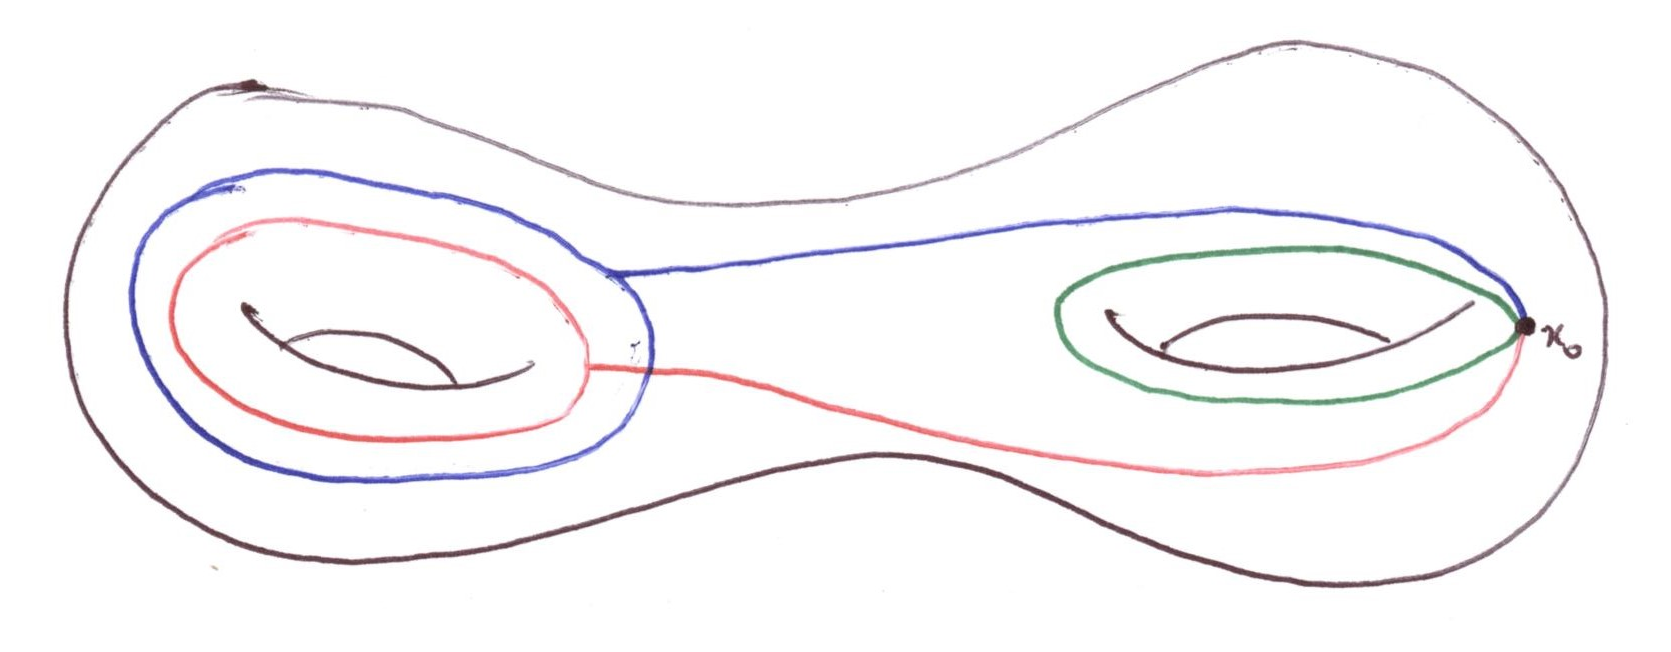
\includegraphics[scale=0.2]{conjugating_loops.png}
\end{figure}

If we have a family of pointed types over a pointed type, i.e. $X:\Type_{\pt}$ and $Y : X \to_{\pt} \Type_{\pt}$, then the type of \emph{pointed sections} is a section $s$ such that $s\ \pt = \pt$, i.e. we only specify this extra data at $\pt : X$. One canonical such section is the constant section $x \mapsto \pt : Y(x)$ and so this is itself a pointed type with the constant section as base point.

There are some lemmas about the levels of connectivity that hold for a space of pointed sections, given data about the connectivity of the base and fibers.

The action of a group $G$ on an object $a : A$ is a map $X: BG \to A$ with $X(pt) = a$. ``Clearly'' this is the same as a homomorphism $G \to \Aut_A a$. (Because a homomorphism is defined as a deloopable map and we just defined the action in terms of the delooping.)

A ``$G$-type'' is a type in the context of $BG$, i.e. a map $X : BG \to \Type$. A map of $G$-types is a function $\alpha : (z : BG) \to X(z) \to Y(z)$. This is a map for each point of $BG$. So we are calling $X$ the $G$-type, not the type $X(pt)$.

Egbert: A higher group $G$ is defined to be a pointed connected type $BG$. The underlying type of the higher group $G$ is then just the loop space of $BG$. This loop space is what $G$ really is, and its group structure comes from it being the loop space of $BG$. A $G$-type should then be a type equipped with a $G$-action. We just define it as a fibration over $BG$, so that the $G$-action comes canonically from the lifting property. So, if $X : BG \to Type$, then we have

- a type $X(*)$ at the base point
- a G-action $X(*) -> X(*)$ for every loop of $BG$

If $X$ would be a $G$-set, then the type of fixed points would be

$$\sum (x : X(*)), \prod (p : * = *), tr(p,x) = x$$

where tr is transport/lift. With a bit of abstract nonsense it follows that this is the type

$$\prod (y : BG), X(y).$$

However, if $X$ is not a $G$-set but a $G$-type, then that first type of fixed points isn't quite right, because it misses the higher coherences. It turns out that the Pi-type is the right thing :)

Greg, later. Given a type family $X$ over a base $BG$, there are two God-given constructions that together produce exactly this fixed-point story. The first is transport: given an equality in the base $x = y$, we get a \emph{function} between fibers $X(x)\to X(y)$. Since the group is the loop space at a point, the transport function is the group action. The second operation is action on paths. Given a \emph{section} $s$  of the type family and an equality $p : x = y$ in the base, we get an equality $tr(p, s(x)) = s(y)$. The narrative with this is that we can't directly compare $s(x)$ and $s(y)$ since they live in different fibers, so first we transport $s(x)$ using $p$ then compare, and we get an equality. In the special case $p : x = x$, i.e. $p \in G$, this is a fixed point for the group action. To recap, given only the group, we only get a function on the fiber (or between fibers if the equality is not a loop). But given also a section, we also get fixed points for the function. This bears further reflection.

So why do we define $X/G := \sum (y : BG), X(y)$? Quotients should have a quotient map: Here the quotient map is just the inclusion of the fiber $X(*)$. The quotient map is surjective: This follows from the fact that $BG$ is connected. The quotient map should be effective: in other words, in $X/G$ we should have

$$q(x)=q(y) \simeq \sum (g:G), gx=y$$

This identity type is a $\Sigma$-type. That's already the first hint that the quotient should be a $\Sigma$-type. And indeed a quick calculation will reveal that effectiveness indeed holds.

Greg, later: ``$gx$'' is the action of $g$, so again transport. So given $p:*=*$ we have $tr_p:X(*) \to X(*)$...

\section{The real outline}
New constructions to import into HoTT: associated bundle, gauge group, Atiyah sequence, flat connection.
\subsection{Associated bundle}
$G$-actions are type families over $BG$, and given $X\to BG$ we can pull any of these back. If we pull back $G$ (as in, the right action of $G$, as a type over $BG$), we get a principal bundle. But if we pull back another action we get the associated bundle. This puts the principal bundle and the associated bundle on the same footing -- they are all actions that we pull back.

A statement to make rigorous: if the image of $X$ is a contractible type containing pt, then the bundle is trivial.
\subsection{Gauge groupoid}
Aka $P\times_G P \to X$. The objects of the groupoid are the fibers of $P$, which of course are in 1-1 correspondence with points of $X$. The morphisms are fiber ismorphisms that are compatible with the $G$-action. This is where holonomy lives. Paths in the manifold give group actions on the fibers of $P$. The path can have separate endpoints and so we examine pairs of fibers.

This specific use of two copies of $P$ only appears when we are implicitly focused on 1-paths which have two endpoints. The right object is probably $\shape P$.

If $P:A\to BG$ is a principal bundle, and given an equality in the base $p: x =_A y$ we get by action-on-paths an equality $P(x)=_{BG}P(y)$ in $BG$, which lifts to any action we may have such as the right action $G$ or $G^{\mathrm{ad}}$.
\subsection{Atiyah sequence}
An exact/fiber sequence of groupoids. (See https://ncatlab.org/nlab/show/Atiyah+Lie+groupoid). Adjoint bundle/groupoid is what Bucholtz et all call $G^{\mathrm{ad}}$. The gauge groupoid is the middle object. And on the right we have $X\times X$, simply pairs of points. We want to replace this with $\shape X$ and so we need a map $\shape X \to X\times X$ and then pull back the diagram.
\subsection{Connection}
A connection is a splitting of the Atiyah sequence. By Schreier theory these are in correspondence with something. A splitting $X\times X \to P\times_G P $ is a trivialization? And a splitting $\shape X \to P\times_G P $ is a flat connection. That's our destination. Meanwhile there's another characterization that uses a map $X\to\flat BG$ to characterize a principal bundle \emph{with} a connection, whereas the principal bundle alone is characterized by $X\to BG$.

In Kolor-Michor-Slovak 9.8 (p. 80) they prove parametrization invariance of transport.
\subsection{Flat connection}
HoTT transport is parallel transport. But HoTT transport operates on equalities instead of paths. The shape modality converts paths into equalities. So given a manifold $X$, we form $\shape X$ and then select a bundle $\shape X \to BG$. Pulling back the right action $G$ type over $BG$, we get a principal bundle. Now any equality in the base can be lifted to an action on fibers and this can directly be interpreted as parallel transport, of a flat connection. We don't have to form the Atiyah sequence and split it, and we don't need the gauge groupoid as of yet. We already have our hands on flat connections just by using standard HoTT transport plus $\shape$.
\subsection{Connections from flat connections}
Here we will work through what Schreiber is saying in DCCT 1.2.7.1.3. Flat 2-connections with values in $\mathrm{INN}G$ model 1-connections and keep track of their curvature. (Schreiber example 1.2.127).

\subsection{Defining the path groupoid in HoTT}
A sub-goal is to define $\textbf{P}(X)$ for a type $X$ using higher inductive types. In Zulip it was suggested I follow the pattern of Licata-Finster when they defined Eilenberg-MacLane spaces. I'm reading the HoTT book chapter 6 and want to read the Cubical materials on HITs as well.

Given a type $X$ we want to set all its paths to equalities, so we will have a constructor that is a function $f:\textbf{P}(X)\to =_X$ where if $p:[0,1]\to X$ then $f(p)\in f(0)=f(1)$. Then we need higher equalities for the thin homotopies, and of course arbitrary non-thin homotopies will not be made into equalities. Perhaps thin homotopies can be described as $n$-homotopies ($n>1$) whose \emph{image} is contained in the \emph{image} of one of the two paths. This will imply that the other path's image is also a subset.

This object can then map to a higher group to create a principal bundle, and transport will be a connection. 

Can I refer to the paths in $X$ as $||\shape X||_1$?

\bibliographystyle{unsrt}
\bibliography{smoothness}

\end{document}
